\chapter{Transformers}

Most competitive neural sequence transduction models have an encoder-decoder structure. The encoder maps an input sequence of symbol representations $x_1, ..., x_n$ (words) to a sequence of continuous representation $ z = z_1, ..., z_n$ (numbers). Given $z$, the decoder then generates an output sequence $y_1, ..., y_m$ of symbols one element at a time. At each step the model is auto-regressive, taking into account the previously generated symbols as additional input when generating the next.

The Transformer follows this overall architecture using stacked self-attention and point-wise, fully connected layers for both the encoder and decoder. Transformers have the advantage over other encoder-decoder based models like LSTM or GRU that they do not use sequential processing and hence they can take advantage of parallel processing and the power of GPUs.

\begin{figure}[h]
    \centering
    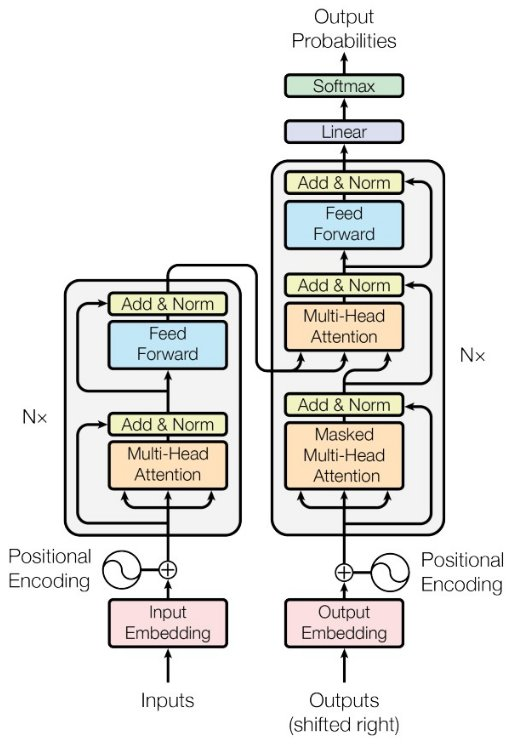
\includegraphics[width=6cm]{Images/trasnformer.jpg}
    \caption{Transformer architecture}
    \label{fig:transformer}
\end{figure}

\noindent Let’s see now the overall transformer architecture in detail which was designed for machine translation:

\newpage
\section{Encoder}

The encoder starts by taking an input sequence of symbol representations $x_1 , ... , x_n$ (words) and transforming them by means of a word embedding process. Basically, this consists in taking the input set of words and encode them as numerical vectors in a way that similar words should have similar representation vectors.

Since the model contains no recurrence (that performs operations in a sequential order) we must add information about the relative or absolute positioning of the words in some way. For this reason we will perform a positional encoding operation to the embedding vectors resulting in an additional positional encoding vector. The result will give us the pre-processed data which will be done only once.

\noindent Now let’s talk about the self-attention mechanism that transformers rely on. Self-attention mechanism is designed to capture relationships between different words in a sequence of text.

Self-attention works first by creating three different copies of the input vector embedding. These three vectors are multiplied by three different weight matrices $W^Q$ , $W^K$ and $W^V$ which weights will be learned during the training process. The result of it will be three different matrices called query $Q= X W^Q$ ,keys $K= X W^K$ and values $V = X W^V$.

\noindent We can use these three matrices to calculate self-attention with the following formula

$$ Attention(Q, K, V) = softmax \left( \frac{Q K^T}{\sqrt{d_k}} \right) V $$

This returns a matrix where each row captures the information from the entire sequence with respect to a single word in the sentence. The importance of each word is weighted according to its attention score.

\noindent Instead of performing a single attention calculation between the query (Q), value (V) and key (K) matrices for a given sequence, the Transformer model employs a multi-head attention mechanism. In multi-head attention, the attention process is carried out multiple times in parallel, with each instance focusing on different learned projections of the query, key, and value vectors. This approach allows the model to capture different types of relationships and patterns in the data simultaneously.

\begin{figure}[h]
    \centering
    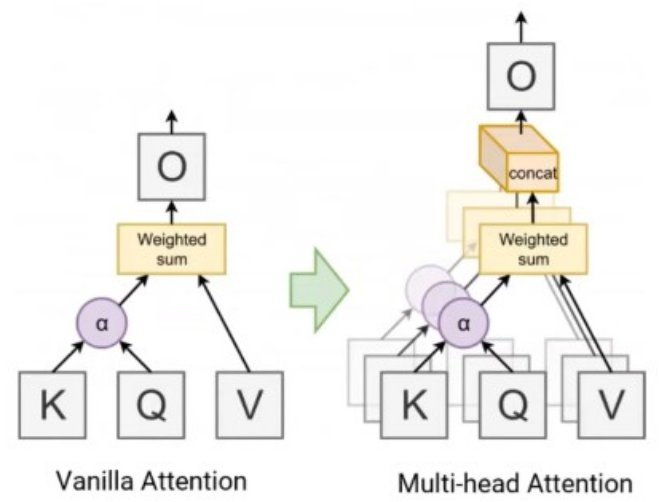
\includegraphics[width=6cm]{Images/self-attention.jpg}
    \caption{Multi-head attention architecture}
\end{figure}

\noindent The attention block is followed by an add and normalization layer. In this layer we first calculate the sum of the output vector of attention block (that we just calculated) and the input embedding vector. The outcome is then subjected to layer normalization (for stable training and better convergence) and passed to the Feed-forward Neural Network for further processing. The purpose of the Feed-forward Neural Network is to process the outcome of one attention layer to better feed the input of the next attention layer.

\newpage
\noindent After the Feed-forward Neural Network there is another add and norm layer that operates in the same way of the one we just described. With this ends the encoder architecture overview. Remember though that the transformer architecture stacks several encoder blocks in top of each other. In the original paper this number was 6.

\begin{figure}[h]
    \centering
    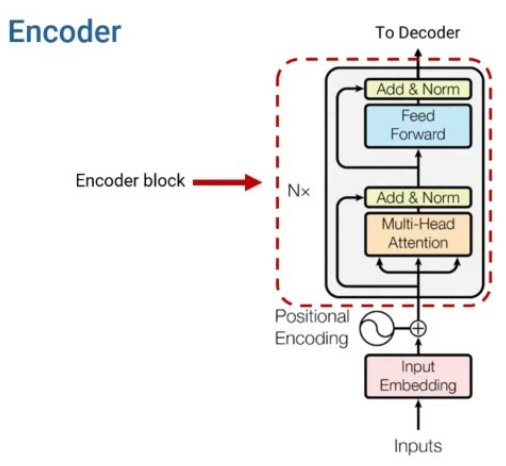
\includegraphics[width=8cm]{Images/encoder.jpg}
    \caption{Encoder architecture}
\end{figure}


\section{Decoder}

Depending if we are performing training or testing the decoder will work in a different way. In training we are fine-tunning the parameters of our model while in testing we will be using the model to actually translate sentences.

\noindent When working in the test mode, we first feed the sentence in one language (e.g English) into the encoder. After the encoder has process the entire sentence this will produce an output which we will feed to the decoder. Based on this output and in previously translated words the decoder chooses the word that is most likely the correct translation (if it is the first word of the sentence a start of the sentence token will be feed instead). This is repeated for every word in the sentence until our decoder decides that the most probable output will be the end of the sentence token. As you could see the encoder uses parallel computing meanwhile the decoder produces outputs one by one during the test phase.

The training phase instead works by using a set of target sentences in order to adjust the parameters of our model so that it would produce the same translation if the same input sentence was given to it. Therefore in training the output translation is available to the model in order to fine tune its parameters.

\begin{figure}[h]
    \centering
    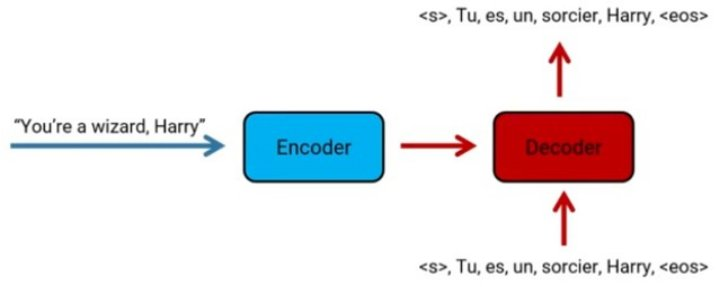
\includegraphics[width=8cm]{Images/translation.jpg}
    \caption{Translation training in the decoder}
\end{figure}

\noindent The embedding and positional encoding steps for the decoder are identical than the ones from the encoder.

\noindent The masked multi-head attention is the first attention layer in the decoder. This layer is similar to the one of the encoder but this time while performing the training (since the input are the target translation) we will be masking the input data of the decoder. This is because we don’t want the transformer to have access to these words as it will harm to its ability to generalize, therefore they are masked by applying a mask matrix on the score.

\begin{figure}[h]
    \centering
    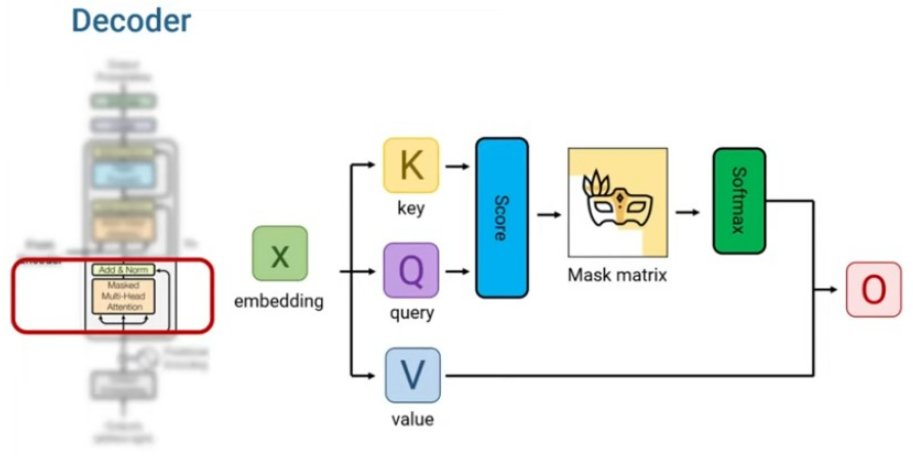
\includegraphics[width=13cm]{Images/masking-decoder.jpg}
    \caption{Masking in self-attention}
\end{figure}

\noindent After this attention layer our data goes through another add and normalization layer. Next, we have a second multi-head attention layer. This is where we finally use the data that the top encoder block produced. In these self-attention layer the keys and values will come from the encoder using the output that encoder gives. Meanwhile the queries will come from the decoder. The decoder takes the target sentence and in the first attention layer produces an attended output. The token that corresponds to the word we are translating is used for the query. The rest of the self-attention process is the same as in the encoder.

\begin{figure}[h]
    \centering
    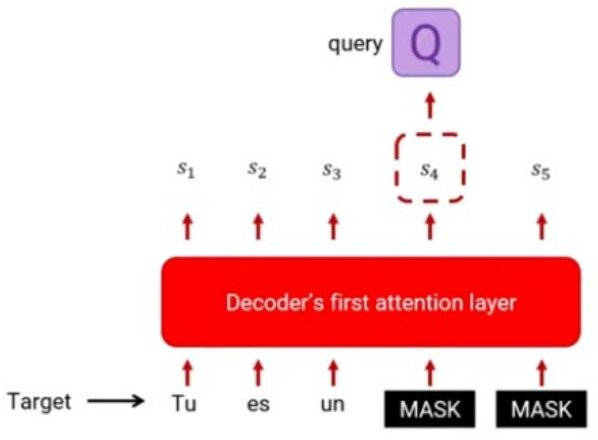
\includegraphics[width=7cm]{Images/decoder-attention.jpg}
    \caption{Decoder attention mechanism}
\end{figure}

\noindent After this comes another add and normalization layer which will work the same as the other ones. The rest of the decoder is very straightforward first we have a feed-forward layer which works the same as in the encoder, then another add and normalization layer, followed by a linear transformation and then a soft-max layer. The soft-max layer will produce the output probabilities.

\newpage
\noindent Finally, keep in mind that the same as in the decoder several decoder blocks are stack in top of each other. In the original implementation of the paper the number of these blocks was 6.

\begin{figure}[h]
    \centering
    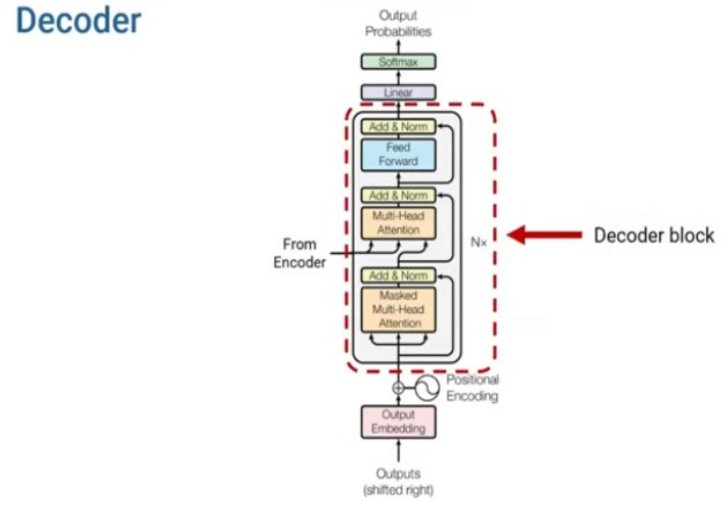
\includegraphics[width=12cm]{Images/decoder.jpg}
    \caption{Decoder architecture}
\end{figure}

\section{Recurrent Neural Networks vs Transformers}

\begin{itemize}
    \item Long Term Dependencies. Recurrent Neural Networks have problems in dealing with long-term dependencies between words that are spread far apart in a long sentence. Transformers do not suffer from this problem, as long as the long-term dependencies are in the range of the maximum allowed input length.
    
    \item Parallel computation. Recurrent Neural Networks process the input sequentially one token at a time: before starting the computation for time step t the computation for time step t+1 should be completed. Meanwhile, transformers can process in parallel all the tokens in the input sequence exploiting matrix multiplication.
    
    \item Context Fragmentation. Attention can only deal with fixed-length sequences, so long sequences should be split into a certain number of segments (chunks) before being fed into a Transformer. This issue doesn't happen in Recurrent Neural Networks.

    \item Out-of-Distribution Generalization. Transformers are not able to implement recurrent rules (if they exist in data), so in principle they do not generalize well to sequences longer than the training ones. Recurrent Neural Networks in principle can learn recurrent rules (if they exist in data).
\end{itemize}




